\documentclass{standalone}
\usepackage{tikz}
\usepackage{ctex,siunitx,bm}
\setCJKmainfont{Noto Serif CJK SC}
\usepackage{tkz-euclide,ninecolors}
\usepackage{amsmath}
\usetikzlibrary{patterns, calc}
\usetikzlibrary {decorations.pathmorphing, decorations.pathreplacing, decorations.shapes,}
\begin{document}
\small
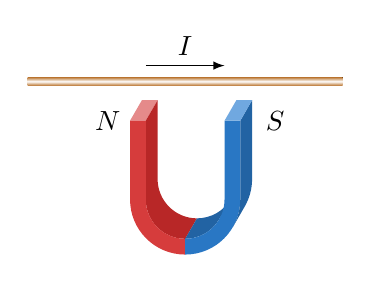
\begin{tikzpicture}[>=latex,yscale=1.0]
  \fill[red7](-0.7,2)--++(0.2,0)--++(60:0.3)--++(-0.2,0)--cycle node[left,text=black]{$N$};
  \fill[red4](-0.5,2)--++(0,-1)arc(180:270:0.5)--++(60:0.3)arc(270:180:0.5)--++(0,1)--cycle;
  \fill[red5](-0.7,2)--++(0,-1)arc(180:270:0.7)--++(0,0.2)arc(270:180:0.5)--++(0,1)--cycle;
  \fill[azure4](0,0.5)arc(270:330:0.5)--++(60:0.3)arc(330:270:0.5)--cycle;
  \fill[azure5](0,0.3)arc(270:360:0.7)--++(0,1)--++(-0.2,0)--++(0,-1)arc(360:270:0.5)--cycle;
  \fill[azure4](0.7,2)--++(0,-1)arc(360:330:0.7)--++(60:0.3)arc(330:360:0.7)--++(0,1)--cycle;
  \fill[azure7](0.7,2)--(0.5,2)--++(60:0.3)--++(0.2,0)--cycle node[right=2mm,text=black]{$S$};
  \draw[->](-0.5,2.7)--(0.5,2.7)node[midway,above]{$I$};
  \fill[top color=brown,bottom color=brown,middle color=white](-2,2.45)rectangle(2,2.55);
\end{tikzpicture}
\end{document}